
%W5100

Η χρήση του ολοκληρωμένου επιλέγεται να γίνει δια μέσω της πλακέτας WIZ811MJ της
ίδιας εταιρείας. Οι λόγοι είναι ότι επιλύει τη διασύνδεση του ολοκληρωμένου με
συνδετήρα RJ-45 (απαραίτητος για την ανταλλαγή δεδομένων μεταξύ W5100 και
δικτύου), ταλαντωτή και διάφορα άλλα ηλεκτρονικά στοιχεία. Από τους 80,
συνολικά, ακροδέκτες του W5100, το WIZ811MJ διαθέτει μόλις 40, οι οποίοι είναι
αυτοί που προορίζονται για τη διασύνδεση με μικροελεγκτή. Όλοι οι υπόλοιποι
συμμετέχουν σε εσωτερικές συνδέσεις της πλακέτας.

Ένα παράδειγμα σχετικά με το τελευταίο, το W5100 διαθέτει έναν ακροδέκτη για το
χειρισμό του ολοκληρωμένου ως Slave σε δίαυλο SPI, το \nbar{SCS}
(\textenglish{SPI Chip-Select}) \parencite[9]{wiz11:w5100}. Ωστόσο, διαθέτει και
έναν επιπρόσθετο ακροδέκτη, τον SEN (\textenglish{SPI Enable}), για την
ενεργοποίηση των υποσυστημάτων του ολοκληρωμένου για λειτουργία σε SPI
\parencite[8]{wiz11:w5100}. Το WIZ811MJ παρέχει ακροδέκτη μόνο για το \nbar{SCS}
ενώ διαθέτει κατάλληλη διάταξη ώστε η αλλαγή της τιμής του να προκαλεί το
αναμενόμενο σήμα στο SEN, αυτομάτως \parencite[7]{wiz13:811mj}.

Επιπλέον σημαντικό χαρακτηριστικό είναι ότι η πλακέτα παρέχει ακροδέκτες
συμβατούς με πρωτότυπες κάρτες (\textenglish{breadboard}) που χρησιμοποιεί η
υλοποίηση, εν αντιθέσει με το W5100 το οποίο είναι SMD
(\textenglish{Surface-Mount Device}) και απαιτεί συγκόλληση
\parencite[6,12]{wiz13:811mj}.

%Αποτελεί μία έτοιμη λύση για την προσθήκη δικτυακών δυνατοτήτων στην υλοποίηση.
%W5100 + MAG-JACK


\subsection{Επικοινωνία με μικροελεγκτή}

Το W5100 υποστηρίζει τρεις τρόπους για την επικοινωνία με το μικροελεγκτή· άμεση
ή έμμεση προσπέλαση ή, μέσω πρωτοκόλλου SPI \parencite[59]{wiz11:w5100}. Οι δύο
πρώτες μέθοδοι χρησιμοποιούν διαύλους διεύθυνσης και δεδομένων απαιτώντας πολλά
σημεία σύνδεσης με το μικροελεγκτή· για την ακρίβεια, 3 γραμμές ελέγχου
(\textenglish{Chip-Select, Read, Write}), 8 γραμμές για το δίαυλο δεδομένων,
και, 15 ή 2 γραμμές διεύθυνσης για άμεση ή έμμεση προσπέλαση, αντίστοιχα. Στην
περίπτωση του SPI απαιτούνται πολύ λιγότερες (μόλις 4) και αυτός είναι ο λόγος
που προτιμάται για τη διασύνδεση του με την MCU, δεδομένου του περιορισμένου
αριθμού ακροδεκτών της. Σαφώς, το μειονέκτημα χρήσης SPI -- ενός σειριακού
πρωτοκόλλου επικοινωνίας -- είναι ότι επιτυγχάνεται πολύ μικρότερος ρυθμός
ανταλλαγής δεδομένων από ότι στην περίπτωση των άλλων δύο, κάτι που, τελικά,
επηρεάζει το χρόνο απόκρισης στα εισερχόμενα αιτήματα. Ωστόσο, κρίνεται ότι για
τις ανάγκες της υλοποίησης, αυτός ο περιορισμός είναι αμελητέος σε σχέση με την
εξοικονόμηση ακροδεκτών που επιφέρει η χρήση SPI.

\begin{figure}
    \caption{Πλακέτα WIZ811MJ και διάταξη των ακροδεκτών του W5100.
    \label{fig:net:811mj-pins}}
    \begin{center}
    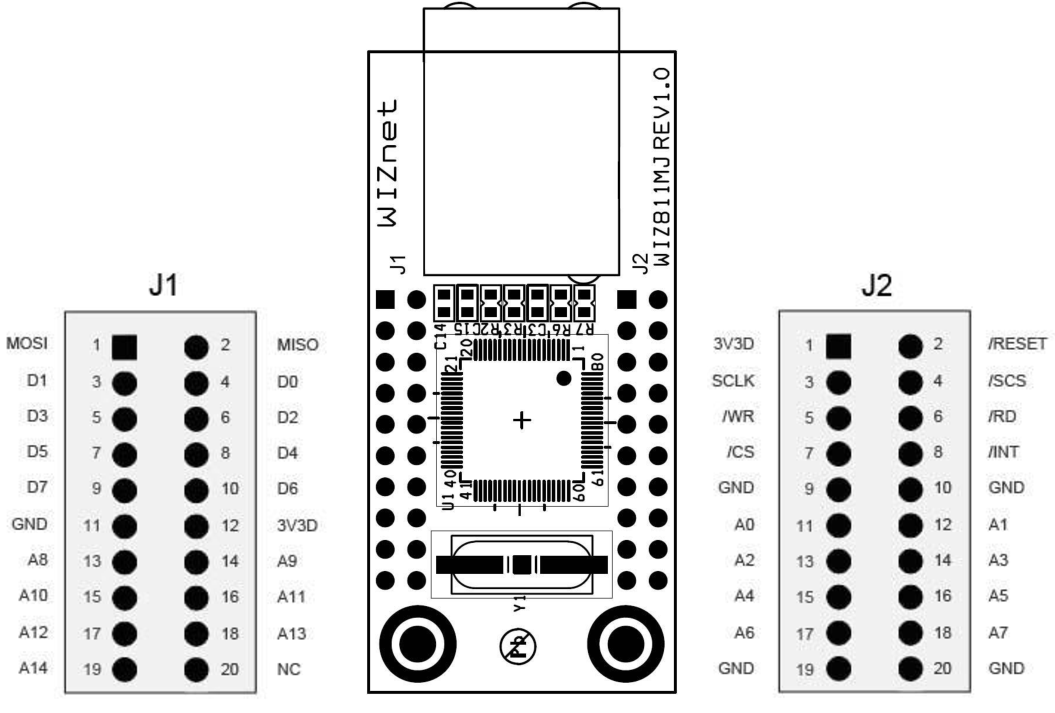
\includegraphics[width=0.9\textwidth]{network_811mj_pin-layout}
    \end{center}
    \fullcite[6]{wiz13:811mj:pins}
\end{figure}

% συνδεσμολογία
Το σχήμα \ref{fig:net:811mj-pins} παρουσιάζει την πλακέτα WIZ811MJ και, σε
μεγέθυνση, την ονομασία των ακροδεκτών της. Από τους ακροδέκτες J1, ιδιαίτερου
ενδιαφέροντος είναι οι 1 (MOSI), 2 (MISO) και 12 (3V3D) εκ των οποίων οι δύο
πρώτοι χρησιμοποιούνται για την μετάδοση των bit του \textenglish{Master} και
του ενεργού \textenglish{Slave} του διαύλου SPI, αντίστοιχα, ενώ ο τελευταίος,
για την τροφοδοσία της πλακέτας με τάση 3.3V. Οι υπόλοιποι, με εξαίρεση τον 20
(\textenglish{Not Connected}), συνδέονται με την τάση αναφοράς, δεδομένου ότι
όλοι, με εξαίρεση τον ακροδέκτη 11 (GND), χρησιμοποιούνται μόνο στην περίπτωση
άμεσης ή έμμεσης προσπέλασης.

Από τους ακροδέκτες J2, ο 1 (3V3D) χρησιμοποιείται για τροφοδοσία 3.3V ενώ οι
9, 10, 19 και 20 (GND) συνδέονται με την τάση αναφοράς. Οι 3 (SCLK) και
(\nbar{SCS}) αποτελούν μέρος του διαύλου SPI για τη μεταφορά του ρολογιού από
το \textenglish{Master} και την ενεργοποίηση του W5100 ως \textenglish{Slave}.
Σύμφωνα με το εγχειρίδιο της \textcite[8]{wiz13:811mj}, ο ακροδέκτης 2
(\nbar{RESET}) προκαλεί την αρχικοποίηση όλων των καταχωρητών του W5100 στις
προεπιλεγμένες τους τιμές και κρίνεται ότι αρκεί να συνδεθεί με το αντίστοιχο
σήμα του μικροελεγκτή ώστε η αρχικοποίηση του W5100 να πραγματοποιείται μαζί
με το μικροελεγκτή.

Οι ακροδέκτες 5 (\nbar{WR}), 6 (\nbar{RD}) και 7 (\nbar{CS}) χρησιμοποιούνται
στην περίπτωση επικοινωνίας μέσω άμεσης ή έμμεσης προσπέλασης και όχι σε SPI
\parencite[8]{wiz11:w5100}. Ωστόσο, επειδή είναι \textenglish{active low},
τίθενται σε μόνιμο λογικό 1 (3.3V), μέσω αντιστάτη, ώστε να είναι λογικά
ανενεργοί.

Μέσω του ακροδέκτη 8 (\nbar{INT}), και εφόσον έχει διευθετηθεί ακολούθως, το
W5100 αναγγέλλει την επιθυμία του για επικοινωνία με το μικροελεγκτή (για
παράδειγμα, επειδή έχουν καταφθάσει δεδομένα). Σε αντίθετη περίπτωση, ο
μικροελεγκτής είναι υποχρεωμένος να εξετάζει από μόνος του το ενδεχόμενο για
επικοινωνία (\textenglish{polling}). Για την υλοποίηση, κρίνεται αξιόλογη η
χρήση των διακοπών. Περισσότερες λεπτομέρειες παρέχονται στην
\nameref{ssubsec:network:ir_imr}.

Για λόγους που έχουν αναφερθεί, όλοι οι υπόλοιποι ακροδέκτες συνδέονται με την
τάση αναφοράς.

Στο σχήμα \ref{fig:network:spi_reset_int} εμφανίζεται η συνδεσμολογία του
μικροελεγκτή με τους ακροδέκτες του W5100 (δια μέσω της πλακέτα WIZ811MJ).
Αξίζει να σημειωθεί ότι, παρόλο που το W5100 λειτουργεί με τάση έως και 3.6V,
ανέχεται τάση στα σήματα εισόδου έως και 5.5V (\textenglish{5V tolerant})
\parencite[64]{wiz11:w5100}. Το χαρακτηριστικό αυτό είναι ιδιαίτερα σημαντικό
επειδή καθιστά δυνατή τη διασύνδεσή του με το μικροελεγκτή χωρίς να απαιτούνται
επιπρόσθετα ενδιάμεσα κυκλώματα για λογικό μετασχηματισμό. %\nref{}

\begin{figure}
    \caption{Διασύνδεση μικροελεγκτή και W5100.
    \label{fig:network:spi_reset_int}}
    \begin{center}
    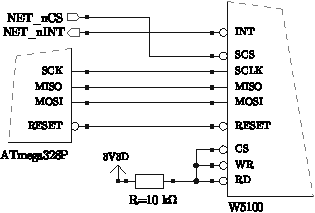
\includegraphics{network_schem_spi_reset_int}
    \end{center}
\end{figure}


\subsection{Διευθέτηση W5100}

Οι καταχωρητές του W5100 χωρίζονται σε δύο κύριες ομάδες· τους καταχωρητές
γενικών ρυθμίσεων (ή κοινοί καταχωρητές) και τους καταχωρητές Socket. Οι κοινοί
καταχωρητές επηρεάζουν τη συμπεριφορά του W5100 συνολικά ή προσδιορίζουν κάποια
χαρακτηριστικά όλων των Socket, ενώ οι καταχωρητές Socket είναι υπεύθυνοι για
τη λειτουργία καθενός εκ των τεσσάρων Socket του ολοκληρωμένου.

Όλοι οι καταχωρητές αντιστοιχίζονται μία διεύθυνση, ενώ υπάρχουν καταχωρητές
περισσοτέρων του ενός byte. Η πρόσβαση σε αυτούς τους καταχωρητές, είτε
πρόκειται για ανάγνωση είτε για εγγραφή, γίνεται από τη χαμηλότερη προς την
υψηλότερη διεύθυνση με \te{Big Endian} διάταξη των byte
\parencite[32--33,35]{wiz11:w5100}.

Οι κοινοί καταχωρητές τίθενται μόνο μία φορά, κατά την εκκίνηση της συσκευής,
και, οι ορισμένοι, κατόπιν εισερχόμενων αιτημάτων (για παράδειγμα, αλλαγή
διεύθυνσης IP). Σε αντίθεση, η πρόσβαση στους καταχωρητές Socket, οι οποίοι
χρησιμοποιούνται για το χειρισμό κάθε Socket, είναι πιο συχνή.


\subsubsection{Καταχωρητές διευθύνσεων και μάσκας υποδικτύου}
\label{ssubsec:network:addr-registers}

Σε αυτήν την κατηγορία συγκαταλέγονται καταχωρητές που ρυθμίζουν τη διεπαφή για
τη σύνδεση με το δίκτυο μέσω των GAR (\te{Gateway Address Register}),
SUBR (\te{Subnet Mask Register}), SHAR (\te{Source Hardware Address Register})
και SIPR (\te{Source IP Address Register}) \parencite[20]{wiz11:w5100}. Η αλλαγή
της τιμής κάποιου, έχει άμεση εφαρμογή στη διεπαφή, γεγονός που λαμβάνεται υπόψη
σε σχετικά εισερχόμενα αιτήματα ώστε να δίνεται απόκριση με τις τρέχουσες
ρυθμίσεις της διεπαφής πριν την ενημέρωσή τους.
% \nref: stored in back-up memory.


\subsubsection{Μέγεθος μνήμης ανά Socket}
\label{ssubsec:network:rmsr_tmsr}

Το W5100 υποστηρίζει μέχρι τέσσερα, ταυτόχρονα, ενεργά Socket καθένα από τα
οποία αποδίδεται ένα μέρος μνήμης από τα συνολικά διαθέσιμα 8KiB για κάθε
κατεύθυνση κίνησης δεδομένων, ανεξάρτητου μεγέθους το καθένα. Οι καταχωρητές
RMSR (\te{RX Memory Size Register}) και TMSR (\te{TX Memory Size Register})
καθορίζουν την προσωρινή μνήμη που αφιερώνεται σε κάθε Socket μεταξύ 1, 2, 4 ή 8
KiB. Σαφώς, πρέπει να δίνεται προσοχή ώστε ο ανατεθειμένος χώρος στα Socket
να μην ξεπερνάει τα 8KiB καθώς, σε αυτήν την περίπτωση, ορισμένα Socket θα
εργάζονται σε κοινές θέσεις στη μνήμη, με ότι επακόλουθα μπορεί αυτό να
επιφέρει.

\begin{figure}
    \caption{Καταχωρητές μεγέθους, RMSR και TMSR.\label{fig:network:rmsr_tmsr}}
    \begin{center}\begin{tabu} spread 0pt {|*8{X[-1,c]|}}

    \hline\rowfont\bfseries
    \multicolumn2{|c}{Socket 3}     &
    \multicolumn2{|c}{Socket 2}     &
    \multicolumn2{|c}{Socket 1}     &
    \multicolumn2{|c|}{Socket 0}   \\

    \hline

    S1  &  S0  &  S1  &  S0  &  S1  &  S0  &  S1  &  S0                       \\
    \hline
    \end{tabu}\end{center}

    Το μέγεθος κάθε Socket καθορίζεται από την τιμή $2^{\text{S1:0}}$.
\end{figure}

Το σχήμα \ref{fig:network:rmsr_tmsr} παρουσιάζει τη σημασιολογία των bit των
δύο αυτών καταχωρητών. Παρατηρείται ότι το μέγεθος της μνήμης κάθε Socket
ρυθμίζεται από δύο, μόνο, bit.
Η υλοποίηση χρησιμοποιεί μόνο ένα Socket με σκοπό τη λήψη και απόκριση αιτημάτων
HTTP. Για το λόγο αυτό οι RMSR και TMSR ρυθμίζονται ώστε να αποδίδονται 8KiB
τόσο για την εισερχόμενη όσο και για την εξερχόμενη προσωρινή μνήμη αποθήκευσης
του Socket 0. Οι ρυθμίσεις του Socket ολοκληρώνονται στην παράγραφο
\nameref{ssubsec:network:port_mr} (σ. \pageref{ssubsec:network:port_mr}).


\subsubsection{Κατάσταση και διακοπές}
\label{ssubsec:network:ir_imr}

Δύο τελευταίοι καταχωρητές που εξετάζονται είναι οι IR(\te{Interrupt Register})
και IMR (\te{Interrupt Mask Register}), οι οποίοι καθορίζουν την κατάσταση
του W5100 και την αναγγελία διακοπών, αντιστοίχως· τα bit του καταχωρητή IR --
μόνο για ανάγνωση -- τίθενται σε κάθε περίπτωση που το απαιτεί, ενώ διακοπή
(μέσω του ακροδέκτη \nbar{INT}) προκαλείται μόνο όταν τίθενται bit του IR των
οποίων το αντίστοιχο bit του IMR έχει, επίσης, τεθεί
\parencite[21--22]{wiz11:w5100}. Με αυτόν τον τρόπο, αναγγέλλονται μόνο οι
διακοπές που ενδιαφέρουν. Επιπλέον, ο μικροελεγκτής εξετάζοντας τον IR μπορεί,
ανά πάσα στιγμή, να αποφασίσει εάν το W5100 χρειάζεται την προσοχή του.

Τα bit των καταχωρητών IR και IMR παρουσιάζονται στο σχήμα
\ref{fig:network:ir_imr}. Από τα συνολικά 7 διαθέσιμα bit, μόνο το S0\_INT που
ειδοποιεί για αλλαγή της κατάστασης του  -- μοναδικού ενεργού -- Socket 0 έχει
ενδιαφέρον για την υλοποίηση και για το λόγο αυτό, τίθεται σε λογικό 1 στον
καταχωρητή IMR. Για λεπτομέρειες σχετικά με τη φύση της διακοπής είναι
απαραίτητη η εξέταση του αφιερωμένου καταχωρητή κάθε Socket.
% \nref: Sn_IR.

\begin{figure}
    \caption{Καταχωρητές κατάστασης και διακοπών, IR και IMR.
    \label{fig:network:ir_imr}}
    \begin{center}\begin{tabu} spread 0pt {|*8{X[-1,C]|}}

    \hline
    \rowfont\bfseries
           7 &       6 &     5 &  4 &       3 &       2 &       1 &       0   \\
    \hline
    CONFLICT & UNREACH & PPPoE & -- & S3\_INT & S2\_INT & S1\_INT & S0\_INT   \\
    \hline
    \end{tabu}\end{center}
\end{figure}

Ένα σημαντικό σημείο είναι ότι το σήμα του ακροδέκτη \nbar{INT} τίθεται και
παραμένει σε λογικό 0 μέχρι να διευθετηθούν όλα τα ενεργοποιημένα, για διακοπή,
bit του IR. Το χαρακτηριστικό αυτό χρησιμοποιείται, στο πλαίσιο της υλοποίησης,
σε συνδυασμό με έναν από τους ακροδέκτες INTn του μικροελεγκτή, ώστε η ρουτίνα
εξυπηρέτησης διακοπής να εκτελείται σε σήμα λογικού 0, και όχι σε παρυφή. Η
διευθέτηση αυτή έχει το πλεονέκτημα ότι ακόμα και εάν ο μικροελεγκτής έχει τεθεί
σε κατάσταση χαμηλής κατανάλωσης (\te{Power-down}), είναι βέβαιο ότι το σήμα
στον \nbar{INT} θα προκαλέσει, εκτός από αφύπνιση της CPU, και την εκτέλεση της
αντίστοιχης ρουτίνας εξυπηρέτησης. Όπως αναφέρεται στο εγχειρίδιο της
\textcite[71]{atmel13}, το τελευταίο είναι κάτι που πρέπει να ληφθεί υπόψη όταν
χρησιμοποιούνται παρυφές για την αφύπνιση καθώς, εάν η διάρκειά τους είναι
σύντομη, παρότι η CPU θα αφυπνιστεί, ενδέχεται να μην αναγνωριστεί η διακοπή.
Έτσι, εξαλείφεται αυτό το ενδεχόμενο.
%\nref : Wake-up from power-down mode.
